%============================================

To set the stage, we record a simple upper bound on grinding power:
\begin{proposition}\label{prop:praos-moments-simple}
  Let $w \in \{0,1\}^n$. Then $g(w) \leq n 2^{\wt(w)}$, where $\wt(w)$ denotes the weight of $w$. If $W$ is distributed according to $B(n,(1 - \epsilon)/2)$ then
  \[
    \Exp[g(W)] \leq n \left(\frac{3 - \epsilon}{2}\right)^n \quad\text{and}\quad\Exp[g(W)^2] \leq n^2\left(\frac{5 - 3\epsilon}{2}\right)^n\,.
  \]
\end{proposition}

\begin{proof}
  Observe that
  \begin{align*}
    \Exp[g(W)] 
    &\leq n\Exp[2^{\wt{W}}] 
    = n\Exp[2^{\sum W_i}] 
    = n\Exp\left[\prod_i 2^{W_i}\right] 
    = n\prod_i \Exp[2^{W_i}] \\
    &= n \left( \frac{1-\epsilon}{2} \cdot 2 + \frac{1 + \epsilon}{2}\right)^n 
    = n \left(\frac{3 - \epsilon}{2}\right)^n\,.
  \end{align*}
    Similarly,
  \[
    \Exp[g(W)^2] \leq n^2 \Exp[2^{2\wt{W}}] = n^2\prod_i \Exp[2^{2W_i}] \leq n^2\left( \frac{1-\epsilon}{2} \cdot 4 + \frac{1 + \epsilon}{2}\right)^n = n \left(\frac{5 - 3\epsilon}{2}\right)^n\,.\qedhere
  \]
\end{proof}

\subsection{Some relaxed bounds on the first and second moments of the grinding power in case of \texorpdfstring{large $\epsilon$}{highly-biased binomial distributions}}
To obtain more precise estimates, for a string $w \in \{0,1\}^*$ define
\[
  t(w) = \begin{cases}
    2^{\wt(w)} & \text{if $\wt(w) \geq |w|/2$\,,}\\
    0 & \text{if $\wt(w) < |w|/2$\,.}
  \end{cases}
\]
Then observe that
\begin{equation}\label{eq:g-decomposition}
  g(w) \leq \sum_{x\; \text{a suffix of $w$}} t(x)\,.
\end{equation}
Intuitively, the quantity $t(w_{n-d+1} \ldots w_n)$ reflects the grinding power of this ``tail'' of the string, equivalent to the number of option sequences for which $i_0 = n-d$ favorably assuming that $w_{n-d} = 0$.
\begin{proposition}\label{prop:moments-general}
  Let $W$ be distributed according to $B(d,(1 - \epsilon)/2)$. Then
  \[
    \Exp[g(W)] \leq \sum_{d = 0}^{n-1} \Exp[t(W_{n-d} \ldots W_n)] \quad \text{and}\quad \Exp[g(W)^2] \leq n \sum_{d = 0}^{n-1} \Exp[t(W_{n-d} \ldots W_n)^2]\,.
  \]
\end{proposition}

\begin{proof}
  The first inequality follows directly from~\eqref{eq:g-decomposition} and the linearity of
  expectation. As for the second inequality, note that if a random
  variable $X$ can be expressed as the sum $Y_1 + \cdots + Y_n$ then
  \[
    \Exp[X^2] = \sum_{ij} \Exp[Y_iY_j] \leq \sum_{ij} \sqrt{\Exp[Y_i^2] \Exp[Y_j^2]} = \left(\sum_i \sqrt{\Exp[Y_i^2]} \right)^2 \leq n \sum_i \Exp[Y_i^2]\,,
  \]
  where both of the inequalities follow from the Cauchy-Schwarz inequality.
  Applying this to the inequality~\eqref{eq:g-decomposition} completes the proof.
\end{proof}

\begin{proposition}\label{prop:moments-t-large-eps}
  Let $W$ be distributed according to $B(d,(1 - \epsilon)/2)$.
  \begin{itemize}
  \item For any $\epsilon \geq 1/3$, \quad $\displaystyle \Exp[t(W)] \leq \left(\sqrt{2(1 - \epsilon^2)}\right)^d\,.$
  \item For any $\epsilon \geq 3/5$, \quad $\displaystyle \Exp[t(W)^2] \leq \left(2\sqrt{1 - \epsilon^2}\right)^d\,.$
  \end{itemize}
  \end{proposition}

\begin{proof}
  Observe that for any $\alpha \geq 1$,
  \[
    \forall w\in \{0,1\}^n \qquad t(w) \leq 2^{(1 - \alpha)d/2 + \alpha\sum_i w_i}\,.
  \]
  It follows that
  \begin{align*}
    \Exp[ t(W) ] &\leq \min_{\alpha \geq 1} \Exp\left[2^{(1 - \alpha)d/2 + \alpha\sum_i W_i}\right] = \min_{\alpha \geq 1} 2^{-(\alpha - 1)d/2} \Exp\left[2^{\alpha\sum_i W_i}\right]\\
                 &= \min_{\alpha \geq 1} 2^{-(\alpha - 1)d/2} \prod_i \Exp\left[2^{\alpha W_i}\right] = \min_{\alpha \geq 1} 2^{-(\alpha - 1)d/2} \prod_i \left[\left(\frac{1+\epsilon}{2}\right) + \left(\frac{1-\epsilon}{2}\right) 2^{\alpha}\right]\\
  &= \min_{\alpha \geq 1} \left(2^{-(\alpha - 1)/2} \left[\left(\frac{1+\epsilon}{2}\right) + \left(\frac{1-\epsilon}{2}\right) 2^{\alpha}\right]\right)^d = \min_{\alpha \geq 1} \left(2^{-1/2} \left[(1+\epsilon)2^{-\alpha/2}  + (1-\epsilon) 2^{\alpha/2}\right]\right)^d\,.
\end{align*}
Considering the quantity
$\beta(a) = (1 - \epsilon) a + (1 + \epsilon) a^{-1}$, note that
\[
  \frac{d\beta(a)}{da} = (1 - \epsilon) - \frac{1 + \epsilon}{a^2}
\]
and hence that $\beta(a)$ is minimized at
\[
  a^*_\epsilon = \sqrt{\frac{1 + \epsilon}{1 - \epsilon}}\,.
\]
Thus the minimum value of $\beta(a)$ is
$2\sqrt{(1 + \epsilon)(1 - \epsilon)}$. When $\epsilon \geq 1/3$, we find that $a_\epsilon^* \geq \sqrt{2}$ which corresponds to a value of $\alpha \geq 1$ above. In this case, 
\[
  \Exp[t(W)] \leq \left( \sqrt{2(1 - \epsilon^2)}\right)^d\,.
\]
The second moment estimate follows from an analogous computation, so
we are more brief. In this case,
  \begin{align*}
    \Exp[ t(W)^2 ] &\leq \min_{\alpha \geq 1} \Exp\left[2^{(1 - \alpha)d + 2\alpha\sum_i W_i}\right] = \min_{\alpha \geq 1} 2^{-(\alpha - 1)d} \prod_i \Exp\left[2^{2\alpha W_i}\right]\\
    &= \min_{\alpha \geq 1} 2^{-(\alpha - 1)d} \prod_i \left[\left(\frac{1+\epsilon}{2}\right) + \left(\frac{1-\epsilon}{2}\right) 2^{2\alpha}\right] = \left(\min_{\alpha \geq 1} \left[(1+\epsilon)2^{-\alpha}  + (1-\epsilon) 2^{\alpha}\right]\right)^d\,.
\end{align*}
As above, this is minimized when $2^\alpha = \sqrt{(1 + \epsilon)/(1 - \epsilon)}$. When $\epsilon \geq 3/5$, the corresponding value of $\alpha$ exceeds $1$ and we conclude that
\[
  \Exp[t(W)^2] \leq \left(2\sqrt{(1 + \epsilon)(1 - \epsilon)}\right)^d\,,
\]
as desired.
\end{proof}

Combining these estimates with Proposition~\ref{prop:moments-general}, we obtain estimates for the first and second moments of $g(W)$. 
\begin{corollary}
  Let $W$ be a random variable distributed according to $B(n,(1-\epsilon)/2)$.
  \begin{itemize}
  \item For any $\epsilon \geq 1/3$, \quad $\displaystyle \Exp[g(W)] \leq \sum_{d=1}^n \left(\sqrt{2(1 - \epsilon^2)}\right)^d\,.$
  \item For any $\epsilon \geq 3/5$, \quad $\displaystyle
    \Exp[g(W)^2] \leq n \sum_{d=1}^n \left(2\sqrt{(1 - \epsilon^2)}\right)^d\,.$
  \end{itemize}
\end{corollary}


These geometric series lead to immediate bounds. 
\begin{corollary} Let $W$ be a random variable distributed according to $B(n,(1-\epsilon)/2)$.
  \begin{itemize}
  \item For any $\epsilon > 1/\sqrt{2}$, \quad
    $\displaystyle
      \Exp[g(W)] \leq \frac{1}{1 - \sqrt{2(1 - \epsilon^2)}}\,.$
  \item For any $\epsilon > \sqrt{3}/2$, \quad $\displaystyle \Exp[g(W)^2] \leq \frac{n}{1 - 2\sqrt{(1 - \epsilon^2)}}\,.$
  \end{itemize}
\end{corollary}

\begin{proof}
  Recall that for $c < 1$, $\sum_{t = 0}^T c^t \leq \sum_{t \geq 0} c^t = 1/(1 - c)$.
\end{proof}

\iftoggle{drawfigs}{

\begin{figure}
  \centering
  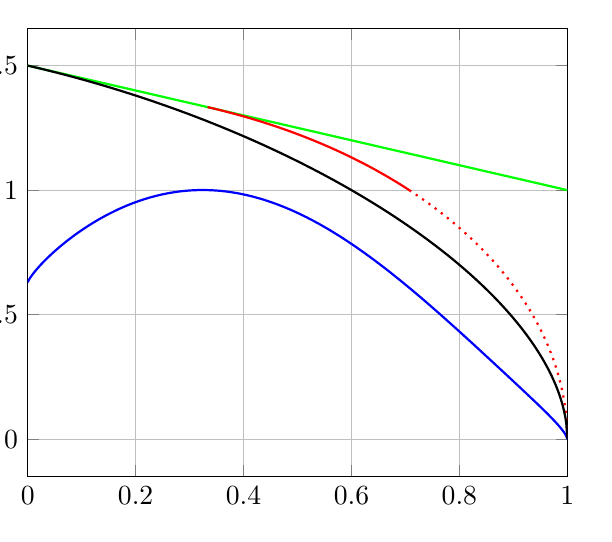
\begin{tikzpicture}[trim axis left,
    declare function={entropy(\x) = - \x * ln(\x)/ln(2) - (1 - \x) * ln(1 - \x) / ln(2); },
%    declare function = { entropy(\x) = 1; },
    ]
    \begin{axis}[domain=0:1,
      samples=500,
      enlarge x limits=false,
      grid=both,
      no markers]
      \addplot +[thick,green] {(3 - x)/2};
      \addplot +[thick,domain=(1/3):(1/1.414),red] {sqrt(2 * (1 - x^2))};
      \addplot +[thick,dotted,domain=(1/1.414):1,red] {sqrt(2 * (1 - x^2))};
      \addplot +[thick,blue] { ((1-x)/2)^(2/3) * (1 + x)^(1/3) * 2^(entropy(x)) };

	  \addplot +[thick,black] {(1-x)/2+sqrt(1 - x^2)};	
	  %\addplot +[thick,black, dotted] { sqrt(2) * (1-x)/2+sqrt(1 - x^2)};	
	  %\addplot +[thick,dotted,black] {(3/2)(1+x)^(1/3)(1-x)^(2/3)};	
\end{axis}
  \end{tikzpicture}
  \caption{(Mean) When $\Exp[g(W)]$ grows exponentially, it is instructive to study the scaled quantity $\mu_1(\epsilon) = \sqrt[d]{\Exp[g(W)]}$. The figure shows a graph of the function $\mu_1(\epsilon)$ in blue, along with the upper bounds on $\mu_1()$ discussed above. The black curve is the asymptotic bound from Claim~\ref{claim:t2star-exact}.}
  \label{fig:grinding-power-mean}
\end{figure}

} % end iftoggle{drawfigs}




%===========================================================


In what follows, we develop tighter bounds via the asymptotics of the binomial coefficients.

\paragraph{Asymptotic bounds on $S(d,z)$.} 
When $z \leq d/3$, the sum $S(d,z)$ will contain the central binomial coefficient ${d-z \choose (d-z)/2}$ which is $\Theta(2^{d-z}/\sqrt{d-z})$. 
It follows that 
\begin{equation} \label{eq:S_d_z_small}
    2^{d-z-1} 
    \leq 
    S(d,z)
    \leq 2^{d-z}\,, 
    \qquad \text{if}\quad 0 \leq z \leq d/3 
    \,.
\end{equation}
On the other hand, for any $0 \leq t < N/2$
\begin{align}\label{eq:binomial-sum-bound}
\frac{2^{H(t/N)N} }{\sqrt{8 (t/N) (1-t/N)} }
\leq 
\sum_{k=0}^t{ {N \choose k} } 
&\leq 
2^{H(t/N)N} \, , 
\end{align}
where $H : [0, 1] \rightarrow [0, 1]$ is the binary entropy function defined as
\begin{align*}
    H(0) &= H(1) = 0\, , \\
    H(\alpha) &= -\alpha \log_2(\alpha) - (1-\alpha) \log_2(1-\alpha)\,, 
        \qquad \text{if}\quad 0 < \alpha < 1\, .
\end{align*}
Thus we can bound $S(d,z)$ using (\ref{eq:binomial-sum-bound}) as follows:
\begin{equation} \label{eq:S_d_z_large}
    \frac{2^{(d-z)H(z/(d-z))}(d-z)}{\sqrt{8 z(d-2z) }}
    \leq
    S(d, z) 
    \leq
    2^{(d-z)H(z/(d-z))}
    \,,\qquad \text{if} \quad d/3 < z \leq d/2 
    \,.
\end{equation}


\subsection{Exact asymptotics for the first moment}
\newcommand{\DoverTwo}{\lfloor d/2 \rfloor}
\newcommand{\DoverThree}{d/3}

In what follows, we establish asymptotically tight upper and lower bounds on 
\begin{align}\label{eq:m_z}
m(d,z) 
&\defeq S(d,z) {d \choose z} \left(\frac{1+\epsilon}{1-\epsilon}\right)^{z} \left(\frac{1-\epsilon}{2}\right)^{d} \, .
\end{align}
via Claims~\ref{claim:t1star-exact} and ~\ref{claim:t2star-exact}. These claims immediately lead to bounds on $\Exp[ g(W) ]$ via Proposition~\ref{prop:grinding-power-mean}.
We also recall the following obvious bound from the sum of a geometric progression:
\begin{align}\label{eq:geom-series-bound}
\sum_{d=1}^n{r^d} 
&\leq \frac{r^{n+1}}{r-1} \qquad \text{if}\quad r > 1\, .
\end{align}





\begin{claim}[Bounds on $m(d,z)$ with small $z$]\label{claim:t1star-exact}
\[
\phi(\epsilon)^d \frac{3}{4\sqrt{d}}
\leq 
m(d, z) 
\leq \phi(\epsilon)^d
\qquad \text{if}\quad z \leq d/3 \quad \text{and}\quad d\geq 2
\]
where $m(d, z)$ is defined in (\ref{eq:m_z}). 
% Moreover, 
% \[
% m(d, z) \leq 1
% \qquad \text{if}\quad z \geq 2\quad \text{and}\quad \epsilon \geq 0.6\,.
% \]
\end{claim}

\begin{proof}
When $z \leq \DoverThree$, we use the upper bound on $S(d,z)$ from (\ref{eq:S_d_z_small}) in (\ref{eq:m_z}) and get
\begin{align*}
m(z)
&\leq 2^{d-z} {d \choose z} \left(\frac{1+\epsilon}{1-\epsilon}\right)^{z} \left(\frac{1-\epsilon}{2}\right)^{d} \\
&= {d \choose z} \left(\frac{1+\epsilon}{2(1-\epsilon)}\right)^{z} (1-\epsilon)^d\,.
\end{align*}
For $z+1 \leq \DoverThree$, the ratio 
\[
\frac{m(z+1)}{m(z)} 
= \frac{d-z}{z+1} \frac{1+\epsilon}{2(1-\epsilon)}
\geq \underbrace{\frac{d-d/3}{\DoverThree}}_{\geq 2} \underbrace{\frac{1+\epsilon}{2(1-\epsilon)}}_{\geq 1/2}
\geq 1\, .
\]
It follows that the sequence $\{m(z)\}$ is an increasing sequence. Consequently,
\begin{align}
m(z; z \leq \DoverThree)
&\leq m(\DoverThree) \nonumber \\
&= {d \choose \DoverThree} (1+\epsilon)^{\DoverThree} (1-\epsilon)^{d- \DoverThree}2^{-\DoverThree} \nonumber \\
&\leq \frac{2^{d H(1/3)}}{\sqrt{\pi (d/3) (2/3)}} 2^{-d/3} (1+\epsilon)^{d/3} (1-\epsilon)^{2d/3} \nonumber \\
&= \left(2^{H(1/3)-1/3} (1+\epsilon)^{1/3} (1-\epsilon)^{2/3} \right)^d \frac{3}{\sqrt{2 \pi d}} \nonumber \\
&= \phi(\epsilon)^d \frac{3}{\sqrt{2 \pi d}} \nonumber \\
&\leq \phi(\epsilon)^d \frac{6}{\sqrt{5 d}} \, . \label{eq:t1star-q1}
\end{align}
Here, we have used Corollary~\ref{coro:nchoosek_1}, the fact that $H(1/3) - 1/3 = \log_2(3/2)$, and (\ref{eq:phi_eps}). This proves the upper bound of the claim. 

% Additionally, since
% \begin{align*}
% \phi(\epsilon) 
% &\defeq \frac{3}{2} (1+\epsilon)^{1/3}(1-\epsilon)^{2/3} \\
% &= \frac{3}{2} \left( (1-\epsilon^2)(1-\epsilon) \right)^{1/3} \\
% &= \frac{3}{2} \left( 1-\epsilon - \epsilon^2 + \epsilon^3 \right)^{1/3} \\
% &= \frac{3}{2}\left( 
% 1 
% + \frac{1}{3}( -\epsilon - \epsilon^2 + \epsilon^3) 
% + \frac{-1}{18}( -\epsilon - \epsilon^2 + \epsilon^3)^2
% + \cdots 
% \right)\\
% &= \frac{3}{2} -\frac{\epsilon}{2} -\left(\frac{1}{2} + \frac{1}{12} \right)\epsilon^2 + O(\epsilon^3) \, ,
% \end{align*}
% $\phi(\epsilon)$ decreases monotonically as $\epsilon$ increases. Hence
% \[
% \phi(\epsilon)\bigg\rvert_{\epsilon \geq 0.6}
% \leq \phi(0.6)
% = \frac{3}{2} (1.6)^{1/3}(0.4)^{2/3}
% = \frac{3}{2}4^{1/3}\frac{4}{10}
% = \frac{3\cdot 4^{1/3}}{5}
% \leq 0.96 < 1\, .
% \]
% This proves the ``moreover'' part of the claim. 

For the lower bound on $m(z)$, apply the lower bound ${N \choose \alpha N} \geq 2^{H(\alpha)N}/\sqrt{8N\alpha (1-\alpha)}$ from Corollary~\ref{coro:nchoosek_1} to the exact expression of $m( \DoverThree)$. This gives 
\begin{align*}
m( \lfloor \DoverThree \rfloor )
&= {d \choose d/3} 
(1+\epsilon)^{d/3} 
(1-\epsilon)^{2d/3} 
2^{-d/3} \nonumber \\
&\geq \frac{2^{d H(1/3)}}{\sqrt{8(d/3)(2/3)}} 2^{-d/3} 
(1+\epsilon)^{d/3} 
(1-\epsilon)^{2d/3} 
\nonumber \quad \text{using Corollary~\ref{coro:nchoosek_1} } \\
&= \frac{3}{4\sqrt{d}}\left(2^{H(1/3) - 1/3} (1+\epsilon)^{1/3} (1-\epsilon)^{2/3}\right)^d \nonumber \\
&= \frac{3}{4\sqrt{d}}\left(\frac{3}{2} (1+\epsilon)^{1/3} (1-\epsilon)^{2/3}\right)^d \\
&= \frac{3}{4\sqrt{d}}\phi(\epsilon)^d \, .
\end{align*}

\end{proof}







\begin{claim}[Bounds on $m(d,z)$ with large $z$]\label{claim:t2star-exact}
\[
\frac{\gamma(\epsilon)^d}{2d}
\leq
m(d, z) 
\leq
\gamma(\epsilon)^d 
% \frac{3\sqrt{d}}{8}
\qquad \text{if}\quad \frac{d}{3} < z \leq \DoverTwo
\, .
\]
where $m(d, z)$ is defined in (\ref{eq:m_z}) and $\gamma(\epsilon) \defeq (1-\epsilon)/2 + \sqrt{1-\epsilon^2}$. Moreover, 
\[
m(d, z) \leq 1
\qquad \text{if}\quad \epsilon \geq 0.6\,.
\]
\end{claim}

\begin{proof}
\textbf{The upper bound.} When $d/3 < z \leq \DoverTwo$, we use the upper bound on $S(d, z)$ from (\ref{eq:S_d_z_large}) into (\ref{eq:m_z}) to get
\begin{align*}
m(z) 
&\leq 2^{(d-z)H(z/(d- z))} {d \choose z} \left(\frac{1+\epsilon}{1-\epsilon}\right)^{z} \left(\frac{1-\epsilon}{2}\right)^{d} \\
&\leq 2^{(d-z)H(z/(d- z)) + H(z/d) d}\left(\frac{1+\epsilon}{1-\epsilon}\right)^{z} \left(\frac{1-\epsilon}{2}\right)^{d}
\end{align*}
using the asymptotic approximation ${N\choose k} \leq 2^{H(k/N)N}$ for $k \leq N/2$. For a fixed $\epsilon$, the function at the exponent of two is concave. There must be some $z^* \in (d/3, \DoverTwo]$ which maximizes $m(z)$. We continue developing the upper bound by setting $\alpha \defeq z/d$. 
\begin{align}
m(z) 
&\leq \left( 2^{q(\alpha, \epsilon)}\right)^d \label{eq:t2star-q2}
\end{align}
where we have defined
\begin{align} \label{eq:q2}
q(\alpha, \epsilon)
& \defeq (1-\alpha) H\left( \frac{\alpha}{1-\alpha} \right) +
H(\alpha) 
-1  + \alpha \log \frac{1+\epsilon}{1-\epsilon} + \log (1-\epsilon)
\end{align}
and $\log$ denotes the base-$2$ logarithm. By applying the definition of $H(.)$,
\begin{align}\label{eq:q2-expanded}
q(\alpha, \epsilon)
&= (1-\alpha) \log\left[
\left( \frac{1-\alpha}{\alpha} \right)^{\frac{\alpha}{1-\alpha} }
\left(\frac{1-\alpha}{1-2\alpha} \right)^{\frac{1-2\alpha}{1-\alpha} }\right] \nonumber \\
& \quad+ \log \left(\frac{1}{\alpha}\right)^\alpha \left(\frac{1}{1-\alpha}\right)^{1-\alpha} \nonumber \\
& \quad+ \log \left(\frac{1+\epsilon}{1-\epsilon}\right)^\alpha + \log(1-\epsilon) -1 \nonumber \\
&= -\log \left[ 
\alpha^{2\alpha} 
(1-2\alpha)^{1-2\alpha} 
\cdot \left(\frac{1-\epsilon}{1+\epsilon}\right)^\alpha 
\right] + \log(1-\epsilon) - 1\, .
% &= 2 a \log(1-2 a)-2 a \log(a)-a \log(1-\epsilon)+\log((-1+\epsilon)/(-2+4 a))+a \log(1+\epsilon)
\end{align}
For a fixed $\epsilon$, this is a unimodal concave function in $\alpha$. The first derivatives of $q(\alpha, \epsilon)$ is
\begin{align*}
\frac{\partial q(\alpha, \epsilon)}{\partial \alpha}
&= \log\left[ \frac{(1-2\alpha)^2}{\alpha^2} \frac{1+\epsilon}{1-\epsilon} \right]
\end{align*}
By setting the above derivative to zero, we find that $q(\alpha, \epsilon)$ is maximized at 
\[
\alpha^* \defeq \alpha^*(\epsilon) 
= \frac{1}{2+\sqrt{\frac{1-\epsilon}{1+\epsilon}} }
= \frac{1}{2+1/r_\epsilon }
= \frac{r_\epsilon}{1 + 2 r_\epsilon }
\]
where we define $r_\epsilon^2 \defeq (1+\epsilon)/(1-\epsilon)$. This means $1-2\alpha = 1/(1+2 r_\epsilon)$. Substituting $\alpha = \alpha^*$ in (\ref{eq:q2-expanded}),
\begin{align*} 
q^*(\epsilon) 
&\defeq q(\alpha^*, \epsilon) \\
&= - \log\left[
\left(\frac{r_\epsilon}{1 + 2 r_\epsilon }\right)^\frac{2 r_\epsilon}{1+2 r_\epsilon}
\left(\frac{1}{1+2r_\epsilon}\right)^\frac{1}{1+2 r_\epsilon}
\cdot \left(\frac{1}{r_\epsilon^2}\right)^\frac{r_\epsilon}{1+2 r_\epsilon}
\right] + \log (1-\epsilon) - 1 \nonumber \\
&= - \log\left[
\frac{1}{1+2 r_\epsilon}
\right] - \log (1-\epsilon) - 1 \nonumber \\
&= \log\frac{1 + 2 r_\epsilon}{1-\epsilon} - 1 \nonumber \\
&= \log\left[\left(1 + 2 \sqrt{\frac{1+\epsilon}{1-\epsilon} } \right) (1-\epsilon) \right] - 1 \nonumber \\
&= \log\left( 1-\epsilon + 2\sqrt{1-\epsilon^2}\right) - 1 \nonumber \\
\implies 2^{q^*(\epsilon)}
&= \frac{1-\epsilon}{2} + \sqrt{1-\epsilon^2}\, .
\end{align*}
This proves the upper bound of the claim. In particular, the derivative of $q^*(\epsilon)$ with respect to $\epsilon$ is $-1/2 - \epsilon/\sqrt{1-\epsilon^2}$. This derivative is negative for all $\epsilon$. Considering that $q^*(0.6) = 1$, it follows that $q^*(\epsilon) < 1$ when $\epsilon > 0.6$. This proves the ``moreover'' part of the claim.

\textbf{The lower bound.} We can use the lower bound on $S(d, z)$ from (\ref{eq:S_d_z_large}) into (\ref{eq:m_z}) to get
\begin{align*}
m(z) 
&\geq 2^{(d-z)H(z/(d- z))}\frac{(d-z)}{\sqrt{8z(d-2z)}} 
{d \choose z} \left(\frac{1+\epsilon}{1-\epsilon}\right)^{z} 
\left(\frac{1-\epsilon}{2}\right)^{d} \\
&\geq 2^{(d-z)H(z/(d- z))}\frac{(d-z)}{\sqrt{8z(d-2z)} } \frac{2^{d H(z/d)} \sqrt{d}}{\sqrt{8z(d-z)} }
\left(\frac{1+\epsilon}{1-\epsilon}\right)^{z} \left(\frac{1-\epsilon}{2}\right)^{d} \qquad \text{using Corollary~\ref{coro:nchoosek_1} on }{d \choose z}\\
&= \frac{\sqrt{d} \sqrt{d-z}}{8z\sqrt{(d-2z)} } 
\left( 2^{q(\alpha, \epsilon)}\right)^{d} \qquad \text{using}\quad \alpha = z/d \quad \text{and} \quad q(\alpha, \epsilon) \text{ from (\ref{eq:q2}) }\\
&= \frac{\sqrt{1-\alpha}}{8\alpha \sqrt{d} \sqrt{(1-2\alpha)} } 
\left( 2^{q(\alpha, \epsilon)}\right)^{d} \\
&\geq \frac{1}{2\sqrt{d}} 
\left( 2^{q(\alpha, \epsilon)}\right)^{d} \qquad \text{since}\quad 1/3 \leq \alpha \leq 1/2\, .
\end{align*}
We have already seen that the right hand side will be maximized by setting
\[
2^{q(\alpha, \epsilon)} \leq \frac{1-\epsilon}{2} + \sqrt{1-\epsilon^2} \qquad \text{for} 1/3 \leq \alpha \leq 1/2, .
\]
This proves the lower bound in the claim.
\end{proof}




% Now we are ready to prove Proposition~\ref{prop:grinding-power-mean}.
% % \restatePropMeanBounds*
% \begin{proof}
% First, note that (\ref{eq:grinding-power-mean-sum}) and (\ref{eq:m_z}) imply that $\Exp[g(W)] = \sum_{d=1}^n{m(d,z)}$. Next, we combine the upper bounds from Claims~\ref{claim:t1star-exact} and \ref{claim:t2star-exact} as $m(d,z) \leq \gamma(\epsilon)^d$ since $\phi(\epsilon) \leq \gamma(\epsilon)$ for $0 \leq \epsilon \leq 1$. This gives $\Exp[ g(W) ] \leq \sum_{d=1}^n{\gamma(\epsilon)^d}$. This is a geometric series; the inequality (\ref{eq:geom-series-bound}) gives the desired upper bound when $\epsilon < 0.6$. At $\epsilon = 0.6$, $\gamma(\epsilon) = 1$; this gives the upper bound of $n$. When $\epsilon > 0.6$, the upper bound is obtained from the geometric-series bound by observing that $\gamma(\epsilon) < 1$.

% The lower bounds for $\epsilon \neq 0.6$ are obtained by summing the geometric series corresponding to the lower bounds from Claims~\ref{claim:t1star-exact} and \ref{claim:t2star-exact}. When $\epsilon = 0.6$, $\gamma(\epsilon) = 1$ and the lower bound is $\sum_{d=1}^n{(1/2d)}$; this equals $1/2$ times the $n$th Harmonic number which, in turn, is at least $\log_e n$. 

% \end{proof}
%--------------------------------------------











% Now we are ready to prove Proposition~\ref{prop:grinding-power-second-moment}
% % \restatePropSecondMomentBounds*
% \begin{proof}
% Recall the inequality $\sum_{d=1}^n{r^d} \leq r^{n+1}/(r-1) = r^n\cdot r/(r-1)$ which follows from the geometric series with $r > 1$. The bounds are obtained by applying this inequality to the upper bounds in Claim~\ref{claim:t1star-variance-exact} and Claim~\ref{claim:t2star-variance-exact}, then making the following observations.
% \begin{align*}
% \frac{5-3 \epsilon}{3-3\epsilon} 
% &\leq 2 \qquad \text{if}\qquad 0 \leq \epsilon \leq 1/3 \\
% \frac{2^{2/3} \phi(\epsilon)}{2^{2/3} \phi(\epsilon) - 1} 
% &\leq 3 \qquad \text{if}\qquad 1/3 < \epsilon \leq 0.6 \\
% \end{align*}

% The last bound follows directly from Claim~\ref{claim:t2star-variance-exact}.
% \end{proof}







%============================================



\subsection{Exact asymptotics for higher moments}
\begin{proposition}\label{prop:grinding-power-moment}
For $t \in \mathbb{N}, t \geq 2$,
\[
\Exp[ g(W)^t ] 
\leq 
(n+3)\left[\frac{1}{2}\left( 2^t + 1 - \epsilon (2^t -1) \right)\right]^n 
\qquad \text{if} \qquad \epsilon \leq \frac{2^t - 2}{2^t + 2}\, .
\]
\end{proposition}
\begin{proof}
Observe that
\begin{align*}
\Exp[ g(W)^t ]
&= \sum_{d = 1}^n{ \Exp[ g(W_{n-d+1}, \cdots, W_n)^t ] }\, ,
\end{align*}
and
\begin{align*}
\Exp[ g(W_{n-d+1}, \cdots, W_n)^t ] 
&= \sum_{z = 0}^{\lfloor d/2 \rfloor} {S(d,z)^t  B(d, (1-\epsilon)/2; z) } \, .
% &= \sum_{z=0}^{\lfloor d/2 \rfloor} {S(d,z)^t {d \choose z} \left(\frac{1+\epsilon}{1-\epsilon}\right)^{z} \left(\frac{1-\epsilon}{2}\right)^{d} }\, .
\end{align*}
Following our own footsteps in arriving at (\ref{eq:q2}), we can write
\begin{align*}
\Exp[ g(W_{n-d+1}, \cdots, W_n)^t ] 
&\leq \sum_{\alpha=0}^{1/3}{2^{t(d-z)} B(d, (1-\epsilon)/2; z) } 
+ \sum_{\alpha=1/3}^{1/2}{2^{t(d-z)H(z/(d-z))} B(d, (1-\epsilon)/2; z) } \\
&= \sum_{\alpha=0}^{1/3}{2^{q_1(\alpha, \epsilon, t)d}} 
+ \sum_{\alpha=1/3}^{1/2}{2^{q_2(\alpha, \epsilon, t)d}} \, ,
\end{align*}
where we have defined
\begin{align} 
q_1(\alpha, \epsilon, t)
& \defeq t(1-\alpha) +
H(\alpha) 
-1  + \alpha \log \frac{1+\epsilon}{1-\epsilon} + \log (1-\epsilon) \label{eq:q1t} \, ,\\
q_2(\alpha, \epsilon, t)
& \defeq t(1-\alpha) H\left( \frac{\alpha}{1-\alpha} \right) +
H(\alpha) 
-1  + \alpha \log \frac{1+\epsilon}{1-\epsilon} + \log (1-\epsilon) \label{eq:q2t}\, .
\end{align}
We calculate the derivatives:
\begin{align*}
\frac{\partial q_1(\alpha, \epsilon, t)}{\partial \alpha}
&= -t 
+ \log \frac{1-\alpha}{\alpha}
+ \log \frac{1+\epsilon}{1-\epsilon} \, ,
\\
\frac{\partial q_1(\alpha, \epsilon, t)}{\partial \alpha}
&= 
(1+t) \log \frac{1-\alpha}{\alpha} 
+ 2 t \log \frac{1 - 2 \alpha}{1 - \alpha}
+ \log \frac{1+\epsilon}{1-\epsilon} \, .
\end{align*}
We observe that $q_1()$ and $q_2()$ agree at $\alpha = 1/3$, as do their derivatives. That is,
\begin{align*}
&q_1(1/3, \epsilon, t) = q_2(1/3, \epsilon, t) \, , \qquad \text{and}\\
&\frac{\partial q_1(\alpha, \epsilon, t)}{\partial \alpha}\bigg\rvert_{\alpha = 1/3}
=
\frac{\partial q_2(\alpha, \epsilon, t)}{\partial \alpha}\bigg\rvert_{\alpha = 1/3}
= 
1 - t + \log \frac{1+\epsilon}{1-\epsilon} \, .
\end{align*}
In addition, $\partial q_1/\partial \alpha$ -- and by equality, $\partial q_2/\partial \alpha$  -- will be non-positive if and only if
\begin{align}
&\epsilon \leq \epsilon^*(t) \defeq \frac{2^t - 2}{2^t + 2} \label{eq:epsstar-moment}
\, .
\end{align}
Notice that we need $t \geq 2$ for $\epsilon^*(t)$ to be meaningful. 

Next, observe that $q_1(\alpha, \epsilon, t)$ is concave in $\alpha$. Suppose $\alpha = \alpha^*$ maximizes $q_1()$. Then, it follows that $q_1(\alpha^*, \epsilon, t) \geq q_1(1/3, \epsilon, t) = q_2(1/3, \epsilon, t) \geq q2(\alpha, \epsilon, t)$. The last inequality follows from the two following facts: that $\partial q_2/\partial \alpha$ is non-positive at $\alpha = 1/3$ and that $q_2()$ is concave in $\alpha$. We can directly solve for $\alpha^*$ by writing \[r_\epsilon \defeq \frac{1+\epsilon}{1-\epsilon}\] and setting
\begin{align*}
&\frac{\partial q_1(\alpha, \epsilon, t)}{\partial \alpha} = 0 \\
\implies& -t 
+ \log \frac{1-\alpha}{\alpha}
+ \log r_\epsilon
=0 \\
\implies& \alpha^* = \frac{1}{1+\frac{2^t}{r_\epsilon}}\, .
\end{align*}
Plugging in $\alpha = \alpha^*$ in (\ref{eq:q1t}), we get
\begin{align*}
q_1(\alpha^*, \epsilon, t)
&= \frac{ \frac{2^t}{r_\epsilon}(t - 1 - \log \frac{2^t}{r_\epsilon} ) - 1 + \log r_\epsilon }{1 + \frac{2^t}{r_\epsilon} }
+ \log \left[ (1-\epsilon) (1+\frac{2^t}{r_\epsilon})\right]\\
&= \log \left[2^t + 1 - \epsilon (2^t -1) \right] - 1\, .
\end{align*}
Thus if we set \begin{align*}
s(\epsilon, t) 
&\defeq 2^{q_1(\alpha^*, \epsilon, t)} \\
&= \frac{1}{2}\left( 2^t + 1 - \epsilon (2^t -1) \right)\, ,
\end{align*}
then
\[
\Exp[ g(W_{n-d+1}, \cdots, W_n)^t ] 
\leq
\frac{d}{2} s(\epsilon, t)^d
\qquad
\text{and}
\qquad
\Exp[ g(W)^t ] 
\leq 
\sum_{d=1}^n{\frac{d}{2} s(\epsilon, t)^d}\, .
\]
It is not difficult to see that for $r> 1$,
\[
\sum_{d=1}^n{d r^d} 
= r \cdot \frac{d}{d r} \left[ \sum_{d=1}^n{r^d}\right] 
\leq \frac{d}{d r} \frac{r^{n+1}}{r-1} 
= \frac{r^{n+1}}{r-1} \left( n + 1 + \frac{r}{r-1}\right) \, ,
\]
where the inequality follows from (\ref{eq:geom-series-bound}). Moreover, If we set $r = s(\epsilon, t)$ in the above equation, we have 
\[
\Exp[ g(W)^t ] 
\leq 
\frac{s(\epsilon, t)^{n+1}}{s(\epsilon, t)-1} \left( n + 1 + \frac{s(\epsilon, t)}{s(\epsilon, t)-1}\right)\, .
\]

\begin{claim}\label{claim:s-ratio}
Equation (\ref{eq:epsstar-moment}) implies
\[
\frac{s(\epsilon, t)}{s(\epsilon, t) - 1 } \leq 2\, .
\]
\end{claim}
Postponing a proof of Claim~\ref{claim:s-ratio} for the moment, we observe that the claim immediately leads to a proof of Proposition~\ref{prop:grinding-power-moment}:
\begin{align*}
\Exp[ g(W)^t ] 
&\leq \sum_{d=1}^n{\frac{d}{2} s(\epsilon, t)^d}\\
&\leq \frac{1}{2} \left[2 s(\epsilon,t)^n ( n + 3) \right] \\
&= (n+3)\left[\frac{1}{2}\left( 2^t + 1 - \epsilon (2^t -1) \right)\right]^n\, .
\end{align*}
It remains to prove Claim~\ref{claim:s-ratio}. Using (\ref{eq:epsstar-moment}), we get
\begin{align}
\frac{s(\epsilon, t)}{s(\epsilon, t)-1}
&= \frac{2^t + 1 - \epsilon(2^t - 1)}{2^t - 1 - \epsilon(2^t - 1)} \nonumber \\
&= 1 + \frac{2}{2^t - 1 - \epsilon(2^t - 1)} \label{eq:claim-s-ratio}
\, .
\end{align}
However, starting from (\ref{eq:epsstar-moment}) we can see that
\[
\epsilon 
\leq 
\frac{2^t - 2}{2^t +2} 
\leq 
\frac{2^t - 5}{2^t - 1}
\leq
\frac{2^t - 3}{2^t - 1}\, .
\]
The last inequality is equivalent to saying $\epsilon(2^t - 1) \leq 2^t - 3$, or $2^t - 1 -\epsilon(2^t - 1) \geq 2$. Referring back to (\ref{eq:claim-s-ratio}), this implies $\displaystyle \frac{s(\epsilon, t)}{s(\epsilon, t)-1} \leq 2$. The proof of Claim~\ref{claim:s-ratio} follows, completing the proof of Proposition~\ref{prop:grinding-power-moment}.
\end{proof}


%------------------- Variance, z > d/3, eps > 0.6 ----------------------
% \textbf{When $\epsilon$ is large.}
% Now consider the case $\epsilon > 0.6$. Setting $\alpha \defeq z/d$ and using the upper bounds from Corollaries ~\ref{coro:nchoosek_1} and \ref{coro:nchoosek_2}, we get
% \begin{align*}
% n(z)
% &\leq a_z \\
% &= 2^{-d}
% (1-\epsilon)^d 
% (d - 2z)^2 
% {d-z \choose z}^2 
% {d \choose z} 
% \left(\frac{1+\epsilon}{(1-\epsilon)}\right)^{z} \\
% &\leq 
% 2^{-d} 
% d^2 
% (1-2\alpha)^2
% 2^{2(1-\alpha)dH(\alpha/(1-\alpha))} \left(\frac{1-\alpha}{\pi d \alpha (1-2\alpha)} \right)
% \frac{2^{H(\alpha)d}}{\sqrt{\pi d \alpha(1-\alpha)}}
% \left(\frac{1+\epsilon}{1-\epsilon}\right)^{\alpha d} (1-\epsilon)^d \\
% &= \frac{\sqrt{d}(1-2\alpha)\sqrt{1-\alpha}}{\pi \alpha \sqrt{\pi \alpha}}
% \left( 2^{H(\alpha) - 1 + 2(1-\alpha) H\left(\alpha/(1-\alpha)\right)} 
% \left(\frac{1+\epsilon}{1-\epsilon}\right)^{\alpha} (1-\epsilon) 
% \right)^d \\
% &\leq \frac{\sqrt{d} }{3} \left( 2^{q(\alpha, \epsilon)} \right)^d\, ,
% \end{align*}
% where
% \begin{align*}
% q(\alpha, \epsilon)
% &\defeq H(\alpha) - 1 + 2(1-\alpha) H\left(\frac{\alpha}{1-\alpha}\right) 
% + \alpha \log \frac{1+\epsilon}{1-\epsilon}+\log(1-\epsilon)\,.
% \end{align*}
% Observe that $q(\alpha, \epsilon)$ is concave in $\alpha$ since for a fixed $\epsilon$, it is a linear combination of the concave entropy function and $\alpha$. The derivatives of $q(\alpha, \epsilon)$, with respect to $\alpha$, are as follows:
% \begin{align*}
% \frac{\partial}{\partial \alpha}q(\alpha, \epsilon)
% &= \log \left(\frac{(1-2\alpha)^4}{\alpha^3(1-\alpha)}  \frac{1+\epsilon}{1-\epsilon} \right)\, .\\
% % \frac{\partial^2}{\partial \alpha^2}q(\alpha, \epsilon)
% % &= -\frac{3-2\alpha}{\alpha(1+2\alpha^2 -3\alpha)} \\
% % \frac{\partial^3}{\partial \alpha^3}q(\alpha, \epsilon)
% % &= \frac{3-2\alpha( 3-2\alpha)^2}{\alpha^2(1+2\alpha^2 -3\alpha)^2} < 0\, .
% \end{align*}

%===========================================================
\subsection{Stirling's approximation and binomial coefficients}
Let us briefly recall an upper bound on binomial coefficients.

\begin{theorem}[Stirling's approximation]
For any positive integer $n$,
\[
n! \, = \, \sqrt{2\pi n}(\frac{n}{e})^n e^{r(n)}\, ,
\]where
\[
\frac{1}{12n} < r(n) < \frac{1}{12n + 1}.
\]
\end{theorem}

Let the binary entropy function $H : [0, 1] \rightarrow [0, 1]$ be defined as
\begin{align*}
H(\alpha) & \defeq \left\{ \begin{array}{ll}0 & \text{ if } \alpha \in \{0, 1\}\\
\\
-\alpha \log_2(\alpha) - (1-\alpha) \log_2(1-\alpha) & \text{ if } \alpha \in (0, 1)\end{array} \right. .
\end{align*}

\begin{corollary}\label{coro:nchoosek_1}
For a positive integer $n$ and any $\alpha \in \{\frac{1}{n}, \frac{2}{n}, \cdots, \frac{1}{2} \}$, 
\begin{align}\label{eq:nck}
  \frac{2^{n H(\alpha)}}{\sqrt{8 n\alpha (1-\alpha)}} 
  \leq {n \choose \alpha n} 
  \leq \frac{2^{n H(\alpha)}}{\sqrt{\pi n\alpha (1-\alpha)}} 
  \leq \frac{2^{n H(\alpha)}}{\sqrt{\pi/2}} \, .
\end{align}
\end{corollary}

\begin{proof}
\begin{align*}
{n \choose \alpha n}
&= \frac{n!}{(\alpha n)!\, \left( (1-\alpha)n \right)! }\\
&\approx \frac{\sqrt{2\pi n}(\frac{n}{e})^n}{2\pi n\sqrt{\alpha (1-\alpha)}(\frac{\alpha n}{e})^{\alpha n}(\frac{(1-\alpha)n}{e})^{(1-\alpha)n} } \underbrace{ \exp\left( \frac{1}{12n} - \frac{1}{12\alpha n + 1} - \frac{1}{12(1-\alpha)n+1}\right) }_{ E(n,\alpha) } \\
&= 2^{n H(\alpha)} \, 1/\underbrace{ \sqrt{2 \pi n\alpha (1-\alpha)} }_{F(n, \alpha)} \, E(n, \alpha) \\
&=2^{n H(\alpha)} E(n, \alpha)/F(n, \alpha) \, .
\end{align*}

\emph{(The upper bounds.)} $E(n,\alpha)$ is at most $e^{1/12 n} < \sqrt{2}$. Hence the first (tighter) upper bound follows. Now we deal with the quantity $F(n, \alpha)/\sqrt{2} = \sqrt{\pi n \alpha (1-\alpha)}$. Since $1-\alpha \geq 1/2$ and $\alpha \geq 1/n$, we have this is at least $ \sqrt{\pi/2}$. \emph{(The lower bound.)} $E(n, \alpha)$ is at least $1$, and $2\pi$ is at most $8$. Hence the bound follows.

\end{proof}

\begin{corollary}\label{coro:nchoosek_2}
For a positive integer $n$ and any $\alpha \in [\frac{1}{n},\frac{1}{2} - \frac{1}{n}]$, 
\begin{align}\label{eq:nck_2}
{(1-\alpha)n \choose \alpha n} \leq 2^{(1-\alpha)n\,H\left( \frac{\alpha}{1-\alpha} \right)}\, G(n, \alpha)\,,
\end{align}
where \[
 G(n,\alpha) \leq \sqrt{\frac{1-\alpha}{\alpha(1-2\alpha) \pi n} } \leq \sqrt{\frac{1-\alpha}{ 2 \pi \alpha} } \leq \sqrt{ \frac{n-1}{2 \pi} }\, . 
 \]
\end{corollary}
\begin{proof}

\begin{align*}
{(1-\alpha)n \choose \alpha n}
&= \frac{((1-\alpha)n)!}{(\alpha n)!\, \left( (1-2\alpha)n \right)! }\\
&\approx \frac{\sqrt{2\pi (1-\alpha)n}(\frac{(1-\alpha)n}{e})^{(1-\alpha)n}}{2\pi n\sqrt{\alpha (1-2\alpha)}(\frac{\alpha n}{e})^{\alpha n}(\frac{(1-2\alpha)n}{e})^{(1-2\alpha)n} } \underbrace{ \exp\left( \frac{1}{12(1-\alpha)n} - \frac{1}{12\alpha n + 1} - \frac{1}{12(1-2\alpha)n+1}\right) }_{E(n,\alpha)}  \\
&= \underbrace{ \sqrt{\frac{1-\alpha}{\alpha(1-2\alpha) 2 \pi n} } }_{F(n, \alpha)}\, \left( \frac{(1-\alpha)^{1-\alpha}}{\alpha^\alpha (1-2\alpha)^{1-2\alpha}} \right)^n\, E(n, \alpha)\\
&=F(n, \alpha) \, 2^{(1-\alpha)n\,H\left( \frac{\alpha}{1-\alpha} \right)} \, E(n, \alpha)\, .
\end{align*}

First, note that $\alpha \leq 1/2 - 1/n$ implies $(1-2\alpha)n \geq 2$. Consequently, $F(n, \alpha) \leq \sqrt{\frac{1-\alpha}{ 4 \pi \alpha} }$. Moreover, $E(n,\alpha)$ is at most $e^{1/12(1-\alpha)n} < \sqrt{2}$. This gives $F(n, \alpha)E(n, \alpha) \leq \sqrt{\frac{1-\alpha}{ 2 \pi \alpha} }$. Since $\alpha \geq 1/n$, the quantity inside the square root is at most $(1-1/n)/2 \pi(1/n) = (n-1)/2\pi$.

\end{proof}
